\documentclass[tikz]{standalone}
\usepackage{tikz}
\usetikzlibrary{shapes.geometric}
\usetikzlibrary{calc}

\begin{document}
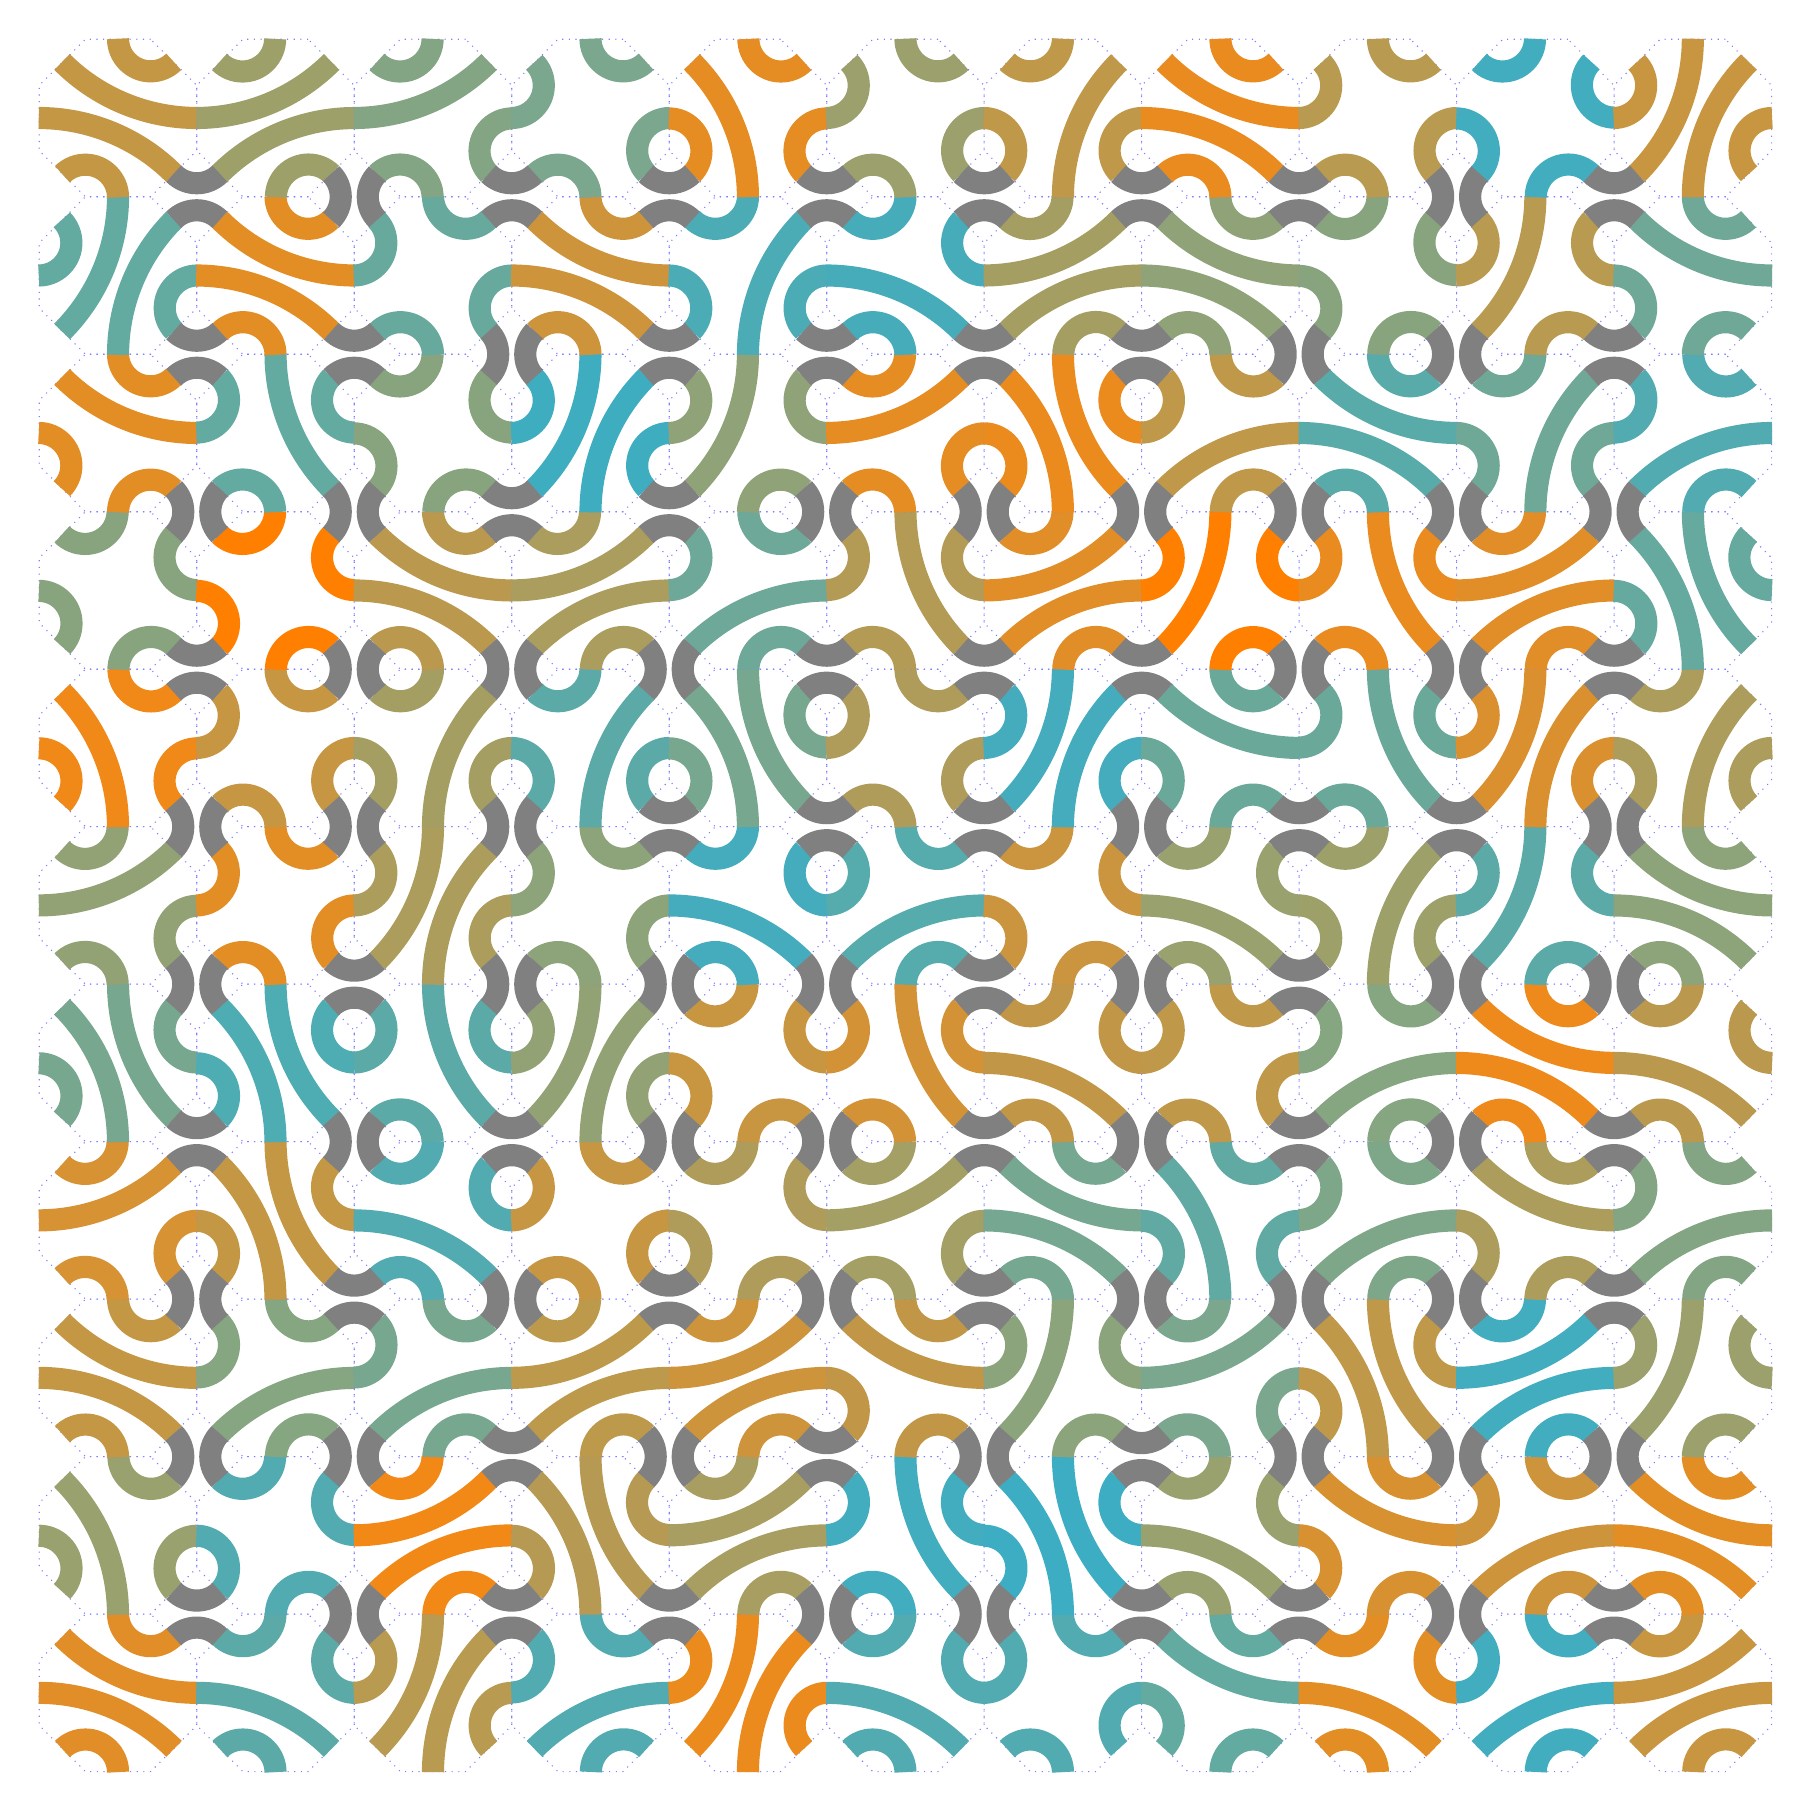
\begin{tikzpicture}
  \newcommand\n{10}
  \node at (0,0) (g) {};
  \foreach \a [evaluate=\x using 2*\a] in {0,...,\n} {
    \foreach \b [
      evaluate=\y using 2*\b,
      evaluate=\r using {random(0,13)},
      evaluate=\s using {random(0,80)}
    ] in {0,...,\n} {
      \node[draw=blue!50, dotted, thin, minimum size=2.1648 cm, regular polygon, regular polygon sides=8] at (\x,\y) (p\a\b) {};
      % \node[minimum size=2.1648 cm, regular polygon, regular polygon sides=8] at (\x,\y) (p\a\b) {};
      \node at (\x,\y) (octagonCenter) {};
      \ifnum \r < 2 {
        % Type I (2 rotations)
        \draw[cyan!\s!orange, line width=8]
          let
            \p{0}=($(p\a\b.corner 3)!0.5!(p\a\b.corner 4)$), % Left
            \p{1}=($(p\a\b.corner 5)!0.5!(p\a\b.corner 6)$), % Bottom
            \p{2}=($(p\a\b.corner 7)!0.5!(p\a\b.corner 8)$), % Right
            \p{3}=($(p\a\b.corner 1)!0.5!(p\a\b.corner 2)$), % Top
          in [rotate around={45*\r:(octagonCenter)}]
          (\p{0}) arc (-90:45:0.4142)
          (\p{1}) arc (0:135:0.4142)
          (\p{2}) arc (90:225:0.4142)
          (\p{3}) arc (180:315:0.4142)
        ;
      } \else {
        \ifnum \r < 6 {
          % Type II (4 rotations)
          \draw[cyan!\s!orange, line width=8]
            let
              \p{0}=($(p\a\b.corner 3)!0.5!(p\a\b.corner 4)$), % Left
              \p{1}=($(p\a\b.corner 5)!0.5!(p\a\b.corner 6)$), % Bottom
              \p{2}=($(p\a\b.corner 7)!0.5!(p\a\b.corner 8)$), % Right
              \p{3}=($(p\a\b.corner 1)!0.5!(p\a\b.corner 2)$), % Top
            in [rotate around={45*\r:(octagonCenter)}]
            (\p{0}) arc (90:45:2.43) % Approximate radius
            (\p{1}) arc (0:135:0.4142)
            (\p{2}) arc (270:225:2.43)
            (\p{3}) arc (180:315:0.4142)
          ;
        } \else {
          % Type III (8 rotations)
          \draw[cyan!\s!orange, line width=8]
            let
              \p{0}=($(p\a\b.corner 3)!0.5!(p\a\b.corner 4)$), % Left
              \p{1}=($(p\a\b.corner 5)!0.5!(p\a\b.corner 6)$), % Bottom
              \p{2}=($(p\a\b.corner 7)!0.5!(p\a\b.corner 8)$), % Right
              \p{3}=($(p\a\b.corner 1)!0.5!(p\a\b.corner 2)$), % Top
            in [rotate around={45*\r:(octagonCenter)}]
            (\p{0}) arc (90:45:2.43) % Approximate radius
            (\p{1}) arc (0:135:0.4142)
            (\p{2}) arc (270:135:0.4142)
            (\p{3}) arc (0:-135:0.4142)
          ;
        } \fi
      } \fi
    }
  }
  \foreach \a [evaluate=\x using 2*\a-1] in {1,...,\n} {
    \foreach \b [
      evaluate=\y using 2*\b-1,
      evaluate=\r using {random(0,1)}
    ] in {1,...,\n} {
      % \draw[red] (\x-0.5858,\y)--(\x,\y+0.5858)--(\x+0.5858,\y)--(\x,\y-0.5858)--cycle;
      \draw[gray, line width=8, rotate around={90*\r:(\x,\y)}]
        (\x-0.2929,\y-0.2929) arc (-45:45:0.4142)
        (\x+0.2929,\y-0.2929) arc (225:135:0.4142)
      ;
    }
  }
  % \node at (5,5) {(5,5)};
  % \node at (4,3) {(4,3)};
  % \node at (1,1) {(1,1)};
\end{tikzpicture}
\end{document}
